\documentclass{report}

% Packages
\usepackage[utf8]{inputenc}

\usepackage{amssymb}
\usepackage{amsmath}
\usepackage{amsthm}
\usepackage{pgfplots}
\newtheorem{Example}{Example}
\usepackage[T1]{fontenc}    % Encodage des polices
\usepackage[english,french]{babel} % Langue du document
\usepackage{subcaption}
\usepackage{hyperref}       % Pour les liens hypertextes
\usepackage{listings}
\usepackage{xcolor}
\newtheorem{theorem}{Theorem}[section]

% Titre du rapport
\title{The Discovery of an  Algebraic structure}
\author{ASSIGBE Komi \\ RAHOUTI Chahid .}
\date{\today}

\begin{document}

\maketitle
\newpage
\tableofcontents

\newpage

\section{Introduction}

\subsection{Definition}
    What is an Algebraic structure? An algebraic structure consists of a nonempty set A (called the underlying set, carrier set or domain), a collection of operations on A (typically binary operations such as addition and multiplication), and a finite set of identities, known as axioms, that these operations must satisfy.

    Among the multiples algebraic structures, we can name:
    \begin{itemize}
        \item Group
        \item Ring
        \item Field
        \item Vector space
                \item .....
            \end{itemize}

        \begin{Example}
            A simple example of a group for 
            addition is the additive group 
            of integers $ (\mathbb{Z}, +) $ 
            satisfies the following properties 
            for any $ a, b, c \in \mathbb{Z} $:
            \begin{itemize}
                \item Closure under the addition operation: $ a + b $ is an integer.
                \item Associativity: $ (a + b) + c = a + (b + c) $.
                \item Existence of the identity element: There exists an element $ 0 \in \mathbb{Z} $ such that $ a + 0 = a $ for every $ a \in \mathbb{Z} $.
                \item Existence of inverses: For each element $ a \in \mathbb{Z} $, there exists an element $ -a \in \mathbb{Z} $ such that $ a + (-a) = 0 $.
                \item Commutativity: $ a + b = b + a $ for every $ a, b \in \mathbb{Z} $.
            \end{itemize}
        These properties make $ (\mathbb{Z}, +) $ a fundamental example of an additive group.
            
        \end{Example}   

\section{Objectives}
    \subsection{Global Objective}

        Our problem is a mathematical problem known 
        as data detection on structured surfaces or 
        varieties.  \\
        With a dataset $V$ 
        defined on a certain surface, the challenge 
        arises in determining whether there exists a 
        discernible algebraic pattern within the data. 
        \\ 
        Essentially, it's about investigating whether 
        there are underlying mathematical relationships 
        or structures governing the given dataset. 
        \\ 
        This problem is crucial in various fields 
        such as algebraic geometry and data analysis, 
        where understanding these structures aids in 
        making predictions or drawing meaningful 
        conclusions from the data.
        \\
        \\
        \\
        \\
        \\
        \\


        \begin{figure}[h]
        \centering
        \begin{tikzpicture}
        \begin{axis}[
            axis lines = middle,
            xlabel = $x$,
            ylabel = {$f(x)$},
            domain=-3:3,
            samples=100,
        ]

        \addplot[blue, thick]{x^3 + x^2};
        \addplot[red, mark = *, only marks] coordinates {(-1,0) (1,2)};
        \addplot[green, mark = *, only marks] coordinates {(2,12)};
        \addplot[dashed, gray] coordinates {(-1,0) (1,2) (2,12)};

        \end{axis}
        \end{tikzpicture}
        \caption{Graphical representation of a 1D dataset $x^3 + x^2$ }
        \end{figure}


    \subsection{Sub Objectives}
        \subsection*{First sub objective: Identify the Best Approch}
        
        They are many ways to attack the problems, one is to consider a group structure on the dataset, then we can define a binary operation on the dataset such that it satisfies the group axioms.
        By this way there are many variables to consider which complicate this approch.
        \\
        The Best way that we choose to attack the problem  is to consider a function $f$ that can map the binary operations defined on $V$ to a binary operation defined on $\mathbb{R}$ that satisfy these two conditions:
        \\
        \begin{theorem}
         \rm{Let $\mathbb{R}$ be the field of real numbers and let $f: \mathbb{R} \rightarrow V$ be a one-to-one function from $\mathbb{R}$ onto a codomain $V$. If we define vector addition by
$$
x \oplus y=f\left(f^{-1}(x)+f^{-1}(y)\right)
$$
and scalar multiplication by
$$
\alpha \odot x=f\left(\alpha \cdot f^{-1}(x)\right)
$$
for all $x$ and $y$ in $V$ and all $\alpha$ in $\mathbb{R}$, then the set $V$, together with the operations $\oplus$ and $\odot$, form a vector space over the field of real numbers.
The real vector space $V$ is sometimes denoted more formally by $(V, \oplus, \odot)$.}
        \end{theorem}
       

        \begin{Example}[Trivial Example]
            Let f be a function from $R$ to $Vect{(e_1)}$ such that $f(x) = x.e_1$.
            we have $f^{-1}(x) = \lambda$.
            we take x and y in $vect{(e_1)}$, we have \\
            $x\oplus y = f(f^{-1}(x) + f^{-1}(y)) = x + y$ \\
            $\alpha \odot x = f(f^{-1}(x) * \alpha) = \alpha x$ 
            \\
            $(Vect{(e_1)}, \oplus, \odot)$ is a vector space
        \end{Example}
        \begin{Example}[Non-Trivial Example]
            Let $\beta$ be any positive real number and let $f: \mathbb{R} \rightarrow \mathbb{R}_{+}^{*}$be
            defined by $f(x)=(1 / \beta) e^x$. Then $f$ is a one-to-one
            function from $\mathbb{R}$ onto the set of positive real numbers, 
            and $f^{-1}(x)=\ln (\beta x)$ for $x>0$. 
            \\
            we would define vector addition and scalar multiplication by :
            \\
            $
            x \oplus y=\frac{1}{\beta} e^{\ln (\beta x)+\ln (\beta y)}=\beta x y
            $
            and
            $
            \alpha \odot x=\frac{1}{\beta} e^{\alpha \ln (\beta x)}=\beta^{\alpha-1} x^\alpha.
            $

            $(R^+, \oplus, \odot)$ is a vector space 

        \end{Example}



        \subsection*{Second sub objective: Implement the 1D case}
            Try to implement a 1D case of the problem, where we have a dataset $V$ defined on a 1D surface.
            \\ 
            We choose this case because, in 1D cas, we can easily evaluate the distance between two points on the dataset based on the norm defined on $\mathbb{R}$.
            \\
            \\
            We will consider this dataset 
            $(\mathbf{x}, \mathbf{x}+\varepsilon \sin (\mathbf{x} / \varepsilon))$ with $\varepsilon \rightarrow 0$.
            \\
            Then we will try to find the best function $f$ that can map the binary operations defined on $V$ to a binary operation defined on $\mathbb{R}$ that satisfy the conditions defined in the first sub-objective.
            \newpage
            \begin{figure}
                \centering
                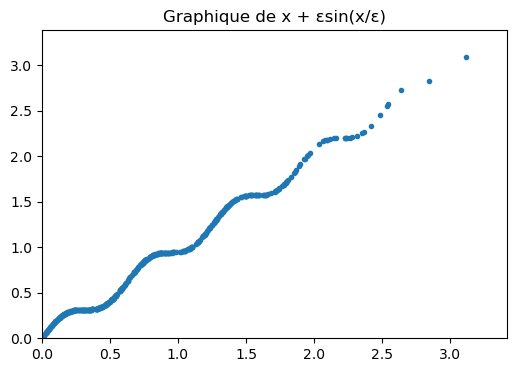
\includegraphics[width=0.5\textwidth]{./images/M.png}
                \caption{Example of 1D dataset  $(\mathbf{x}, \mathbf{x}+\varepsilon \sin (\mathbf{x} / \varepsilon))$ with $\varepsilon \rightarrow 0$, we took $\varepsilon = 0.1$ and x randomly choose following a normal distribution with mean 0 and variance 1.} 
            \end{figure}

        \subsection*{Third sub objectif : 3D case}
        \subsection*{Third sub objectif : 3D case}
            Here, we will consider a dataset $V$ defined on a 2D surface.

        
<<<<<<< HEAD
<<<<<<< HEAD
\section{Mathematical setting}
=======
\section{Mathematical analysis}
>>>>>>> 290c6fe (Changes and New Result)
=======
\section{Mathematical analysis}
>>>>>>> 290c6fe (Changes and New Result)
    To address these objectives, we leverage
    the Pytorch library in Python using Neural Networks Learning to find the optimal parameters that minimize the loss function.\\
    We are also going to use also Git to share Code and collaborate on the project.\\ 
    We will also use slack for communication and sharing information.\\

    As said in  First sub-Objective, if we consider An algebraic structure like a group, this is our we attack the problems, we transform the a group axioms into a loss to minimize we can define the losses as follows : 
    As said in  First sub-Objective, if we consider An algebraic structure like a group, this is our we attack the problems, we transform the a group axioms into a loss to minimize we can define the losses as follows : 

    \begin{enumerate}
        \item Existence of the identity element:  \[
            L_1(\theta) = \sum_{v \in V} (e_{\text{obs}} - e_{\text{pred}})^2
            \]
        \item Commutativity:
        \[
        L_2(\theta) = \sum_{(x, y) \in V \times V} (x \oplus y - y \oplus x)^2
        \]
        \item Associativity:
        \[
        L_3(\theta) = \sum_{(x, y, z) \in V \times V \times V} ((x \oplus y) \oplus z - x \oplus (y \oplus z))^2
        \]
        \item Existence of inverses:
        \[
        L_4(\theta) = \sum_{x \in V} (-x_{\text{obs}} + (-x_{\text{pred}}))^2
        \] 
    \end{enumerate}
    
    Here, $\theta$ represents the parameters of our model.
    These functions $L_i(\theta)$ measure the discrepancies
    between the observed and predicted values for each group 
    axiom, where $i = 1, 2, 3, 4$. By minimizing these functions
    $L_i(\theta)$, we aim to adjust our model to be as close as
    possible to the real data, ensuring that our algebraic 
    structure accurately satisfies the group axioms. 

    $$
    L(\theta) = \min_{\theta} L_1(\theta) + L_2(\theta) + L_3(\theta) + L_4(\theta)
    $$


    This function $L(\theta)$ represents the sum of losses 
    associated with each group axiom. By minimizing 
    this function $L(\theta)$, we aim to adjust our model so
    that it optimally satisfies the four group axioms, 
    ensuring the accuracy and consistency of our 
    algebraic structure with respect to the provided data.\\

    \textbf{Like, there are many unknows parameters to consider, that why we choose to consider attack the problem using the definition based on a Vector space.}\\

    
    Here is the approch that we will use to attack the problem using the definition based on a Vector space:


    \begin{enumerate}
        \item Loss for vector addition:
        \[
            L_1(\theta) = \sum_{(x, y) \in V \times V} \left\lVert x \oplus y - \left(f(f^{-1}(x)) + f(f^{-1}(y))\right) \right\rVert_{V}^2
            L_1(\theta) = \sum_{(x, y) \in V \times V} \left\lVert x \oplus y - \left(f(f^{-1}(x)) + f(f^{-1}(y))\right) \right\rVert_{V}^2
        \]
        \item Loss for scalar multiplication:
        \[
            L_2(\theta) = \sum_{(\alpha, x) \in \mathbb{R} \times V} \left\lVert \alpha \odot x - f(\alpha \cdot f^{-1}(x)) \right\rVert_{V}^2
            L_2(\theta) = \sum_{(\alpha, x) \in \mathbb{R} \times V} \left\lVert \alpha \odot x - f(\alpha \cdot f^{-1}(x)) \right\rVert_{V}^2
        \]
    \end{enumerate}

    Function $L(\theta)$, the sum of these two functions:
    \[
    L(\theta) = L_1(\theta) + L_2(\theta)
    \]

    We  precise that the norm $\left\lVert \cdot \right\rVert_{V}$ is the norm defined on the dataset $V$.
    We  precise that the norm $\left\lVert \cdot \right\rVert_{V}$ is the norm defined on the dataset $V$.

\section{Tools}
    We use Neural Networks Learning to find the best couple that minimize the loss function $L(\theta)$.
    We use the Pytorch library in Python to implement the algorithms and the Neural Networks Learning, and Git, slack to share and communicate on the project.
\section{Tools}
    We use Neural Networks Learning to find the best couple that minimize the loss function $L(\theta)$.
    We use the Pytorch library in Python to implement the algorithms and the Neural Networks Learning, and Git, slack to share and communicate on the project.

\section{Base Algorithms}
    For reaching the objectives, which we have defined, here is the algorithms we implement in our projet  : 
    The algorithms have been implemented in Python using the Pytorch library and the Neural Networks Learning.\\
    \begin{enumerate}
        \item \textbf{Morphism}: This class defines a morphism from 
        $\mathbb{R}^n$ to a space $E$ with dimension $dim_E$. 
        It consists of three fully connected layers, each with 
        a specified number of neurons. The forward function computes 
        the output of the morphism given an input $x$.
        \item \textbf{InverseMorphism}: This class defines an inverse
        of function $f: E \rightarrow \mathbb{R}^n$. It consists of
        three fully connected layers, each with a specified number
        of neurons. The forward function computes the output of the
        inverse morphism given an input $x$.
        \item \textbf{LoiBinaire}: This class defines a binary operation 
        between two elements $x$ and $y$ in $E$. It consists of three 
        fully connected layers, each with a specified number of neurons. 
        The forward function computes the output of the binary operation 
        given two inputs $x$ and $y$.
        \item \textbf{LoiScalaire}: 
        This class defines a scalar operation between a scalar $\alpha$ and an element $x$ in $E$. A scalar operation is an operation that combines a scalar and a vector to produce a new vector. In the context of neural networks, this could mean an operation such as scalar multiplication. This class consists of four fully connected layers, each with a specified number of neurons. The forward function computes the output of the scalar operation for a scalar $\alpha$ and an input $x$. The scalar $\alpha$ is multiplied by $x$ to produce a new vector $z$, which is then passed through the layers of the network to produce the output.
        \item \textbf{Vect\_space} : This class defines a vector space $E$ with dimension $\dim{E}$. It consists of a morphism, an inverse morphism, a binary operation, and a scalar operation. 
        \\ 
        It contains the Train function that trains the model to minimize the loss function $L(\theta)$. It updates the network's weights to minimize the loss function, using the provided optimizer. 
    \end{enumerate}


\section{Numerical Experiments}
    We choose to consider a dataset  which is almost an affine manifold because, in this case, we can easily evaluate the distance between two points on the dataset based on the norm defined on $\mathbb{R}$. It is the first easiest way to tackle the problem and to understand the behavior of the model.\\
    And also we can use the binary operations defined on the dataset to define the binary operations on $\mathbb{R}$.

    \subsection{Numerical Experiments}
        \subsubsection{One Dimensional Case}
            We consider the dataset $(\mathbf{x}, \mathbf{x}+\varepsilon \sin (\mathbf{x} / \varepsilon))$ with $\varepsilon \rightarrow 0$.
            \\
            The data used :
            \begin{itemize}
                \item $\mathbf{x}$ is randomly chosen following a normal distribution with mean 0 and variance 1.
                \item $\varepsilon = 0.1$
                \item  $dim_E = 2$ like the dataset is defined on a 2D 
                        surface have 2 dimensions, the abscissa and the ordinate.
                \item The Number of Epochs = 1000  to train the model.
                \item The learning rate = 1e-3
                \item  $dim_E = 2$ like the dataset is defined on a 2D 
                        surface have 2 dimensions, the abscissa and the ordinate.
                \item The Number of Epochs = 1000  to train the model.
                \item The learning rate = 1e-3
            \end{itemize}
        % -----------------------------
        \subsubsection{Results}
            After, the model is trained, we have those results :
            For the Losses, we have 
            \begin{table}[h]
                \centering
                \begin{tabular}{|c|c|c|c|}
                \hline
                Epoch & L_{1} & L_{2} & L = L_{1} + L_{2} \\
                \hline
                0/1000 & 27.517923 & 27.298063 & 54.815987 \\
                200/1000 & 7.004137 & 2.402620 & 9.406757 \\
                400/1000 & 0.815794 & 0.108183 & 0.923977 \\
                600/1000 & 0.027651 & 0.014956 & 0.042607 \\
                800/1000 & 0.020693 & 0.014033 & 0.034726 \\
                0/1000 & 27.517923 & 27.298063 & 54.815987 \\
                200/1000 & 7.004137 & 2.402620 & 9.406757 \\
                400/1000 & 0.815794 & 0.108183 & 0.923977 \\
                600/1000 & 0.027651 & 0.014956 & 0.042607 \\
                800/1000 & 0.020693 & 0.014033 & 0.034726 \\
                \hline
                \end{tabular}
                \caption{Training results with 64 neurons per layer for the Loss}

                \caption{Training results with 64 neurons per layer for the Loss}

            \end{table}

            % -----------------------------
            % let plot the graph of the Losses par une figure
            \begin{figure}[h]
                \centering
                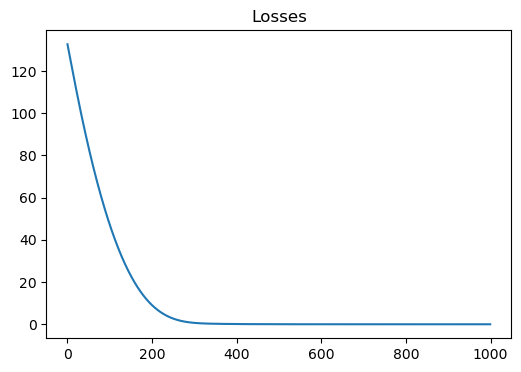
\includegraphics[width=\textwidth]{./images/losses.png}
                \caption{Losses during training}
                \label{fig:losses}
            \end{figure}

            % -----------------------------
            \newpage

            % -----------------------------

            % let plot the graph of the dataset and the predicted dataset
            We have noticed that the Loss decreases as the number of epochs increases, which indicates that the model is learning and improving its performance over time. The total loss is the sum of the two individual losses, which are also decreasing as the model is trained. This suggests that the model is effectively minimizing the loss function and optimizing the parameters to better fit the data.

        \subsubsection{Validation Test}
            It consist to test the model on a new dataset that the model has never seen before. So we choose some points belonging to a dataset (points that is not the training dataset) and we apply the binary operations defined on the dataset to verify the properties of the Vect space. \\
            It means that, for two points in $V$, the Direct sum of these two points will be equal to the morphism of the sum of the inverse morphism of these two points. And for a scalar $\alpha$ and a point in $V$, the scalar multiplication of the point will be equal to the morphism of the scalar multiplication of the inverse morphism of the point.

            Let choose Five points belonging to the Dataset: \\
            \begin{table}[h]
                \centering
                \begin{tabular}{|c|c|c|c|c|}
                \hline
<<<<<<< HEAD
<<<<<<< HEAD
                B\_x & B\_y & C\_x & C\_y & \alpha \\
=======
                B\_x & B\_y & C\_x & C\_y & alpha \\
>>>>>>> 290c6fe (Changes and New Result)
=======
                B\_x & B\_y & C\_x & C\_y & alpha \\
>>>>>>> 290c6fe (Changes and New Result)
                \hline
                -0.801354 & -0.900084 & -0.358002 & -0.315550 & 0.1384 \\
                -0.475507 & -0.375598 & -0.077409 & -0.147315 & 0.6890 \\
                -0.962686 & -0.942615 & -0.838647 & -0.924802 & 0.6502 \\
                -0.084069 & -0.158579 & -0.069757 & -0.133992 & 0.5863 \\
                -0.487856 & -0.389233 & -0.498922 & -0.402730 & 0.8824 \\
                \hline
                \end{tabular}
                \caption{Points belonging to the dataset}
                \end{table}
            

            % -----------------------------

            \newpage
            After we apply the binary operations defined, we have the following results :\\

            \begin{tabular}{|c|c|c|}
                \hline
<<<<<<< HEAD
<<<<<<< HEAD
                f(f^{-1}(B) + f^{-1}(C)) & B$\oplus$C & L^2 Erreur  \\
=======
                f.fi(B) + f.fi(C) & B$\oplus$C & Erreur \\
>>>>>>> 290c6fe (Changes and New Result)
=======
                f.fi(B) + f.fi(C) & B$\oplus$C & Erreur \\
>>>>>>> 290c6fe (Changes and New Result)
                \hline
                0.009636102, -0.1696734 & 0.008442776, -0.16858363 & 1.6e-03 \\
                0.011397708, -0.17639658 & 0.007390147, -0.17639616 & 4.0e-03 \\
                0.0076359604, -0.1628094 & 0.004921416, -0.16270462 & 2.7e-03 \\
                0.012931213, -0.18012077 & 0.013284955, -0.18060187 & 6.0e-04 \\
                0.009761432, -0.17229007 & 0.0035657752, -0.16988468 & 6.6e-03 \\
                \hline
            \end{tabular}
<<<<<<< HEAD
<<<<<<< HEAD
=======
=======
>>>>>>> 290c6fe (Changes and New Result)
            \\
            \\
            $f$ is the morphism \\
            $fi$ is the inverse morphism.
<<<<<<< HEAD
>>>>>>> 290c6fe (Changes and New Result)
=======
>>>>>>> 290c6fe (Changes and New Result)

            % -----------------------------
            Let see illustrate the results by a figure :
            \begin{figure}[h]
                \centering
                \begin{minipage}{0.5\textwidth}
                \begin{minipage}{0.5\textwidth}
                    \centering
                    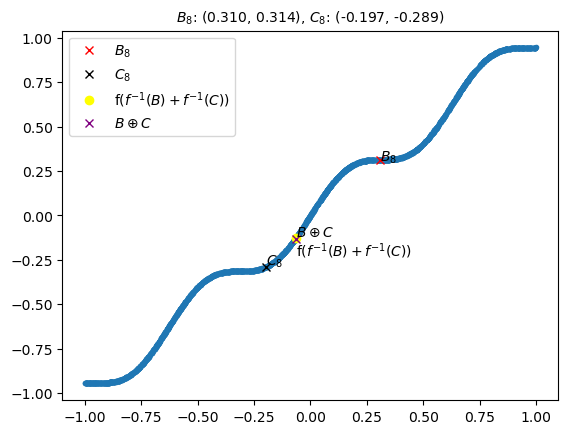
\includegraphics[width=0.9\linewidth]{./images/1.png}
                \end{minipage}%
                \begin{minipage}{0.5\textwidth}
                    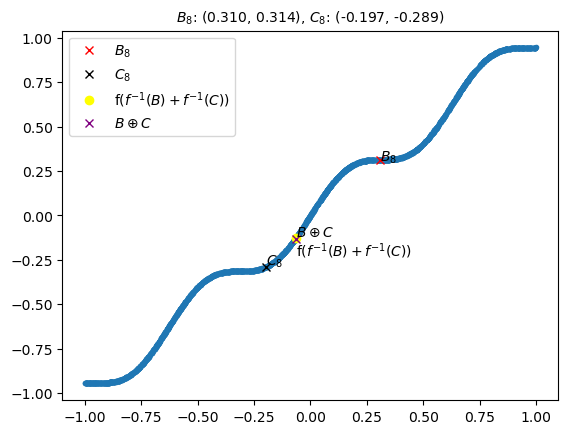
\includegraphics[width=0.9\linewidth]{./images/1.png}
                \end{minipage}%
                \begin{minipage}{0.5\textwidth}
                    \centering
                    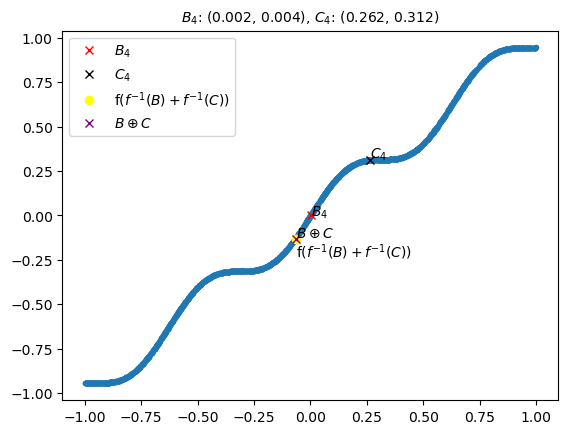
\includegraphics[width=0.9\linewidth]{./images/2.png}
                \end{minipage}
                    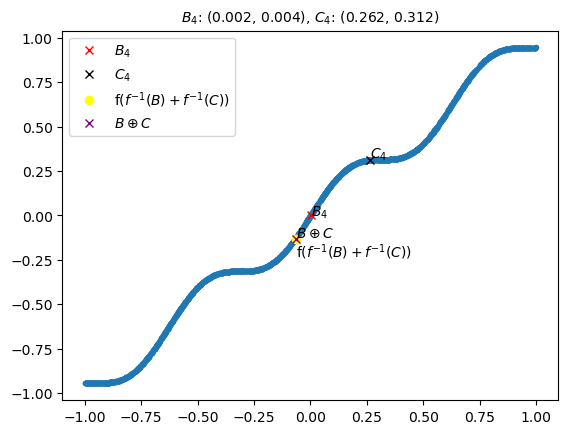
\includegraphics[width=0.9\linewidth]{./images/2.png}
                \end{minipage}
            \end{figure}
            
            \begin{figure}[h]
                \centering
                \begin{minipage}{0.5\textwidth}
                    \centering
                    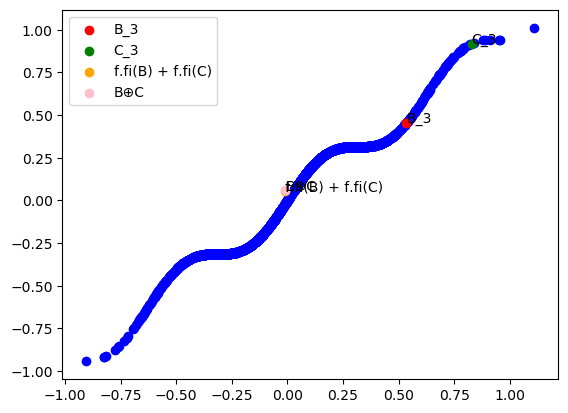
\includegraphics[width=0.9\linewidth]{./images/3.png}
                \end{minipage}%
                \begin{minipage}{0.5\textwidth}
                    \centering
                    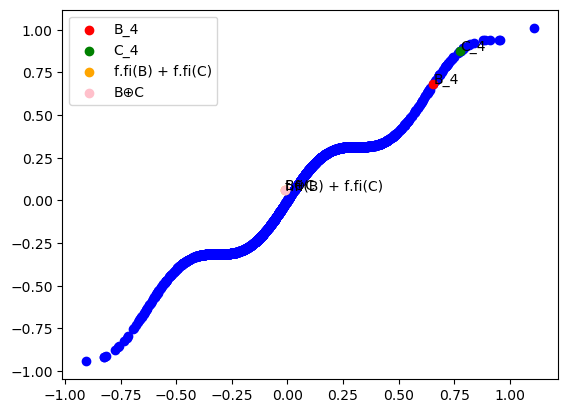
\includegraphics[width=0.9\linewidth]{./images/4.png}
                \end{minipage}
            \end{figure}
            

            \begin{figure}[h]
                \centering
                \begin{minipage}{0.5\textwidth}
                    \centering
                    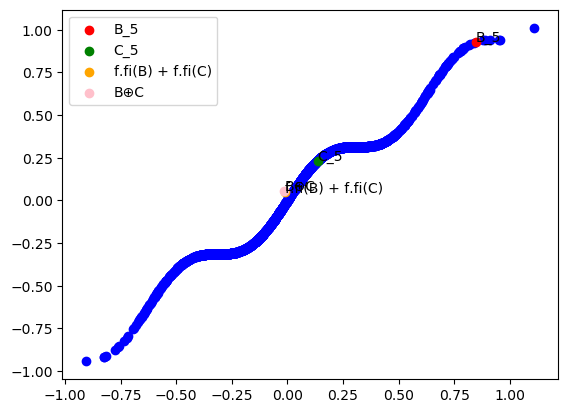
\includegraphics[width=0.9\linewidth]{./images/5.png} % Remplacez par le chemin de votre image
                \end{minipage}%
                \begin{minipage}{0.5\textwidth}
                    \centering
                    % Espace vide pour aligner l'image sur la gauche
                \end{minipage}
            \end{figure}

            \newpage


            Doing the same thing for the scalar multiplication, we have the following results:\\

            \begin{tabular}{|c|c|c|}
                \hline
<<<<<<< HEAD
<<<<<<< HEAD
                f(\alpha . fi(B)) & \alpha \odot B & L^2 erreur \\
=======
                f(alpha * fi(B)) & alpha * B & Erreur \\
>>>>>>> 290c6fe (Changes and New Result)
=======
                f(alpha * fi(B)) & alpha * B & Erreur \\
>>>>>>> 290c6fe (Changes and New Result)
                \hline
                0.073016845, 0.07753995 & 0.07003992, 0.0773815 & 3.0e-03 \\
                0.07220963, 0.07294881 & 0.06926333, 0.07280513 & 2.9e-03 \\
                0.0706523, 0.06543551 & 0.06751147, 0.065266766 & 3.1e-03 \\
                0.0702148, 0.06404036 & 0.06719723, 0.06386372 & 3.0e-03 \\
                0.07182709, 0.07203528 & 0.06874711, 0.071856365 & 3.1e-03 \\
                \hline
            \end{tabular}
            \\

            Here is the illustration for the scalar multiplication :
            \begin{figure}[h]
                \centering
                \begin{minipage}{0.5\textwidth}
                    \centering
                    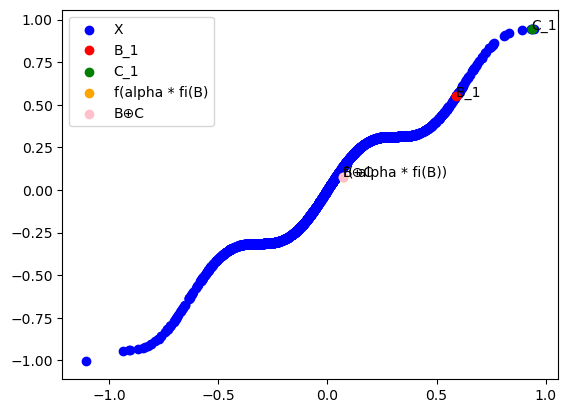
\includegraphics[width=0.9\linewidth]{./images/alpha1.png}
                \end{minipage}%
                \begin{minipage}{0.5\textwidth}
                    \centering
                    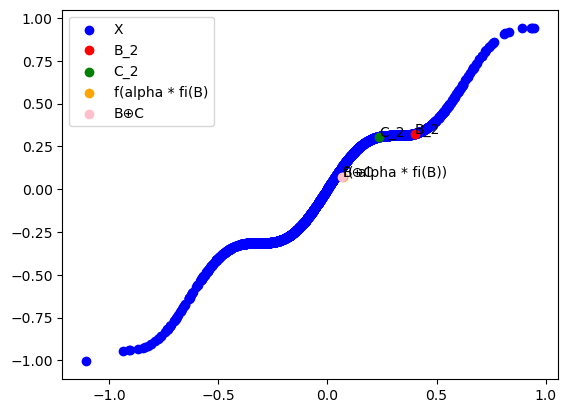
\includegraphics[width=0.9\linewidth]{./images/alpha2.png}
                \end{minipage}
            \end{figure}
            
            \begin{figure}[h]
                \centering
                \begin{minipage}{0.5\textwidth}
                    \centering
                    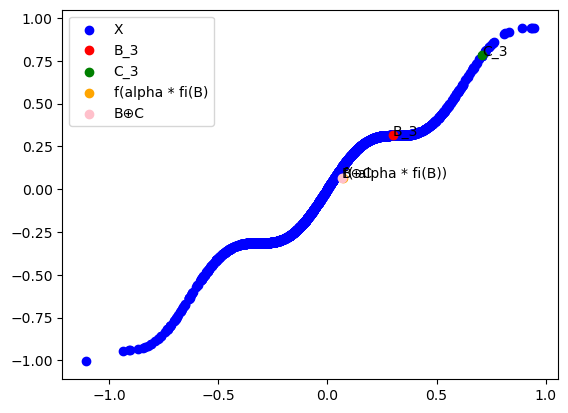
\includegraphics[width=0.9\linewidth]{./images/alpha3.png}
                \end{minipage}%
                \begin{minipage}{0.5\textwidth}
                    \centering
                    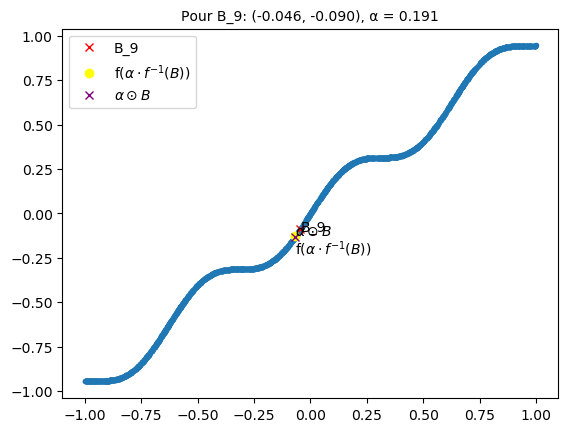
\includegraphics[width=0.9\linewidth]{./images/alpha4.png}
                \end{minipage}
            \end{figure}
            

            \begin{figure}[h]
                \centering
                \begin{minipage}{0.5\textwidth}
                    \centering
                    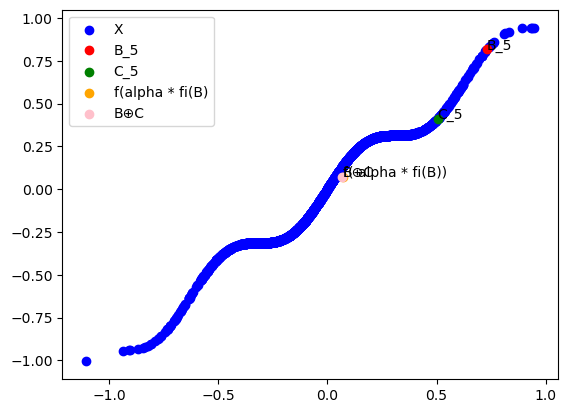
\includegraphics[width=0.9\linewidth]{./images/alpha5.png} % Remplacez par le chemin de votre image
                \end{minipage}%
                \begin{minipage}{0.5\textwidth}
                    \centering
                    % Espace vide pour aligner l'image sur la gauche
                \end{minipage}
            \end{figure}
        \newpage


<<<<<<< HEAD
<<<<<<< HEAD
        \textbf{As conclusion, we see that the error between the Direct Sum and the morphism of the sum of the inverse morphism is to ordre 3, and the error between the scalar multiplication and the morphism of the scalar multiplication of the inverse morphism is also to ordre 3 . This means that the model is effectively learning the properties of the vector space and accurately reproducing the binary operations defined on the dataset.\\
=======
        \textbf{As conclusion, we see that the error between the Direct Sum and the morphism of the sum of the inverse morphism is very small, and the error between the scalar multiplication and the morphism of the scalar multiplication of the inverse morphism is also very small. This means that the model is effectively learning the properties of the vector space and accurately reproducing the binary operations defined on the dataset.\\
>>>>>>> 290c6fe (Changes and New Result)
=======
        \textbf{As conclusion, we see that the error between the Direct Sum and the morphism of the sum of the inverse morphism is very small, and the error between the scalar multiplication and the morphism of the scalar multiplication of the inverse morphism is also very small. This means that the model is effectively learning the properties of the vector space and accurately reproducing the binary operations defined on the dataset.\\
>>>>>>> 290c6fe (Changes and New Result)
        So we can conclude that (V, $\oplus$, $\odot$) is a vector space with an algebraic structure.}


\section{General Manifolds}








            













\section{Application}
Many differential equations encountered 
in solving have parametric solutions.
Thus, to find the solution for each 
parameter, this often requires 
numerous calculations. To optimize 
computation and storage times, we 
define an algebraic structure 
whereby, if we compute the solution 
for parameters $\lambda_1$ and $ \lambda_2 $,
we can deduce $\lambda_3$ ...
\begin{Example}
    Consider the general form of a first-order linear ODE with a parameter $\lambda$:
    
    \[
    \frac{dy}{dx} + \lambda y = 0
    \]
    
    The solution to this differential 
    equation depends on the parameter
    $\lambda$, the solution to this ODE is given by:
    
    \[
    y(x) = C e^{-\lambda x}
    \]
    where $C$ is the constant of integration.
    The solution on $y(0)=1$ is given by:
    $y(x) = e^{-\lambda x}$
    

\begin{tikzpicture}
\begin{axis}[
    axis lines = middle,
    xlabel = $x$,
    ylabel = {$y(x)$},
    domain=0:3,
    samples=100,
    legend pos=outer north east
]

\addplot[blue, thick]{exp(-0.5*x)}; \addlegendentry{$\lambda = 0.5$}
\addplot[red, thick]{exp(-3*x)}; \addlegendentry{$\lambda = 3$}
\addplot[green, thick]{exp(-7*x)}; \addlegendentry{$\lambda = 7$}

\end{axis}
\end{tikzpicture}


In this example, the parameter $\lambda$ affects the behavior of the solution function $y(x)$. Different values of $\lambda$ lead to different solutions, each with its own characteristic behavior. Thus, the solution is a function with a parameter $\lambda$.
\end{Example}

\section{Conclusion}
this project provides a comprehensive 
exploration of algebraic structures and
their relevance in data analysis, 
offering insights into how these 
structures can be effectively applied 
to detect patterns and derive meaningful
conclusions from datasets. Through Python 
implementation and testing, the project 
demonstrates practical approaches to 
optimize algebraic structures for 
improved accuracy and performance 
in various applications
    
\end{document}